\documentclass[tikz,border=2pt]{standalone}
\renewcommand{\familydefault}{\sfdefault}
\usetikzlibrary{arrows.meta,calc,positioning}
\tikzset{every picture/.style={line width=1pt, >=Stealth},
         hl/.style={fill=black, fill opacity=0.12, text opacity=1}}
\begin{document}
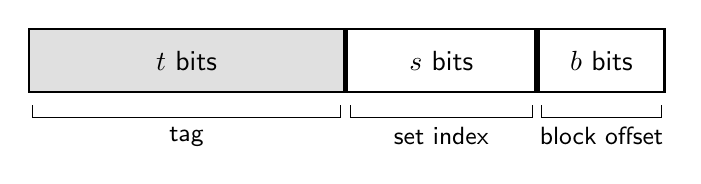
\begin{tikzpicture}[field/.style={draw, minimum height=0.8cm, anchor=west}]
  % An address splits into three fields, most significant on the left.
  \node[field, hl, minimum width=4cm] (t) at (0, 0) {$t$ bits};
  \node[field, minimum width=2.4cm] (s) at (t.east) {$s$ bits};
  \node[field, minimum width=1.6cm] (b) at (s.east) {$b$ bits};
  \foreach \f/\name in {t/tag, s/set index, b/block offset} {
    \draw[thin] ([shift={(0.06, -0.15)}]\f.south west) -- ++(0, -0.15) -| ([shift={(-0.06, -0.15)}]\f.south east);
    \node[below, font=\small] at ([yshift=-0.3cm]\f.south) {\name};
  }
\end{tikzpicture}
\end{document}
